\section{Results}
\label{chap:results}

\end{multicols}
\begin{figure}[t]
	\centering
	\includegraphics[width=1\linewidth, keepaspectratio]{tech_comp.eps}
	\caption{comparing various ways in which the q-EELS data can be extracted from the EFTEM stack}
	\label{fig:tech-comp}
\end{figure}%
%
\subsection{Comparing data extraction techniques}
In figure \ref{fig:tech-comp} three different q-EELS maps are plotted, the radial, linear and slicing technique from top to bottom respectively. It is immediately obvious that the radial and linear "integration" techniques have higher resolutions along the momentum transfer axis. This is due to the fact that slicing the EFTEM stack between two points yields a pixelated line, similarly to opening paint and drawing a line, whereas the integration techniques also extract information from pixels just besides the line between two points resulting in smaller momentum transfer steps. One drawback to these techniques is that they also add intensity values from pixels not directly between to diffraction spots to the q-EELS map, this is especially so with the radial integration technique that uses all values on a circle outwards from the starting point.
The integration techniques also yield a smoother gradient from low-$q_{\perp}$ to high-$q_{\perp}$ since it averages multiple q-EELS spectra in a ringsize, this again might introduce spectra not truly on the line in between two points but does average out any unwanted errors such as external radiation.\\
\newpage
%
%
\begin{figure}[t]
	\centering
	\includegraphics[width=1\linewidth, keepaspectratio]{qmap_corr_comp.eps}
	\caption{Batson correction for q-EELS map}
	\label{fig:bat-cor}
\end{figure}
%
\subsection{Reviewing Batson correction}
Carrying out the Batson correction on the sliced q-EELS map of the $\Gamma$-InSe sample in the $\gamma \rightarrow M \rightarrow K$-direction we can clearly see it has a big effect on the map. The q-EELS spectra near the low momentum transfer $\Gamma$-point are nearly fully erased. This was to be expected as it was also reported by earlier work.\cite{Schneider:191230} Amplifying this region was not the intention of applying the Batson correction since the original EFTEM stack's data was sufficient. The high momentum transfer region near the high symmetry $M$- and $K$-points has benefitted from the correction, the q-EELS spectra had their zero-loss peaks removed and contrast heightened making it easier to resolve features in these spectra.\\
An apparent but not unexplainable feature or artefact of the correction is the dark band in the middle between the $M$- and $K$-points. The original q-EELS map (top figure in \ref{fig:bat-cor}) had a bright spot in the middle of the zero-loss peak at the same position, the Batson correction uses an integral of the intensity over the zero-loss peak to scale the to be subtracted correction spectrum. Thus if there is an extra bright feature in the zero-loss peak the correction spectrum gets improperly scaled to be to large for what it needs to correct for and will upon subtraction remove to much intensity from the rest of the spectrum.\\
Another dark shadow can be seen spanning the whole momentum transfer range at about $14eV$ energy loss. This darker streak seems to curve upwards towards the middle and come back down, trailing nearly perfectly the bulk plasmon dispersion. This streak can not be explained by the subtraction since it curves upwards and the correction spectrum is subtracted centred around the zero-loss peak which curves downward towards negative energy losses.\\
The zero-loss peak itself is removed nicely from the q-EELS map for a majority of the momentum transfers. The Batson correction seems to leave a bit of the zero-loss peaks for moderately low momentum transfers. This could be due to the fact that the Batson correction uses a simulated image spectrum for its correction which underrepresents the zero-loss peak. A simulated image spectrum is used for the reasons outlined in \ref{sec:batsen} and might not be accurate enough as Batson himself reported in his work \cite{PhysRevB.27.5224}. It could also be that the sum of smaller intense dispersions remains in the low-loss region. This would be hard to tell without a higher energy resolution.\\
Some more Batson corrected q-EELS maps have been included in the appendix \ref{fig:bat-cor-comp}.
\newpage
%
\begin{figure}[t]
	\centering
	\includegraphics[width=1\linewidth, keepaspectratio]{qmap_peak.eps}
	\caption{tracked peaks on stitched q-EELS map}
	\label{fig:qmap-track}
\end{figure}
%
\subsection{Interesting features from data}
%
For tracking the peak of the bulk plasmon a high enough separation between the peak and background spectrum was needed. The q-EELS map in figure \ref{fig:qmap-track} was made by stitching together the uncorrected q-EELS map in the low momentum transfer regime and the Batson corrected q-EELS map for high momenta transfers. The q-EELS data was gathered using the slicing method from the $\Gamma$-point to $M$, then $K$, and back to $\Gamma$ with the definition of the points the same as earlier q-EELS maps and consistent with figure \ref{fig:tr-diff-im}.\\
The energy loss value of the plasmon peak was found by searching for the highest intensity value in a window around a centre energy loss value, this method does not always find the true peak as the outliers both far above and below the central point cloud show. The values for the peak of the plasmon were scrubbed from outliers and plotted in the bottom plot of figure \ref{fig:qmap-track}, a sine centred around the point in the middle of the $M$ and $K$ lines was fitted and provides a decent result around the middle but deviates from the true function at the $\Gamma$-lines.\\
%
\begin{multicols}{2}
\begin{figure}[H]
	\centering
	\captionsetup{width=0.8\linewidth}
	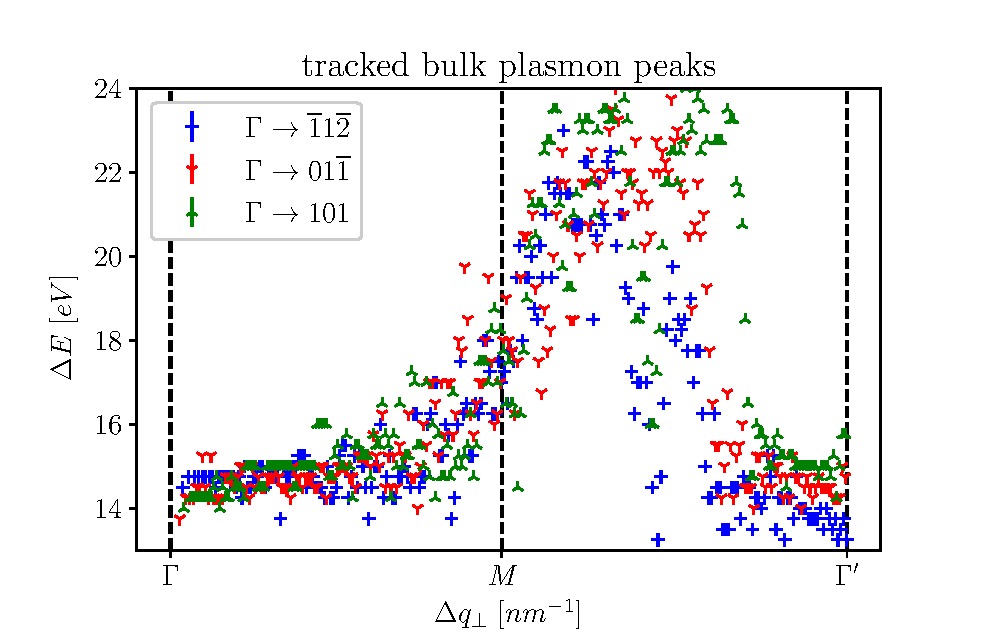
\includegraphics[width=1\linewidth, keepaspectratio]{plasmon_dispersion.eps}
	\caption{tracked peaks of the plasmon dispersion.}
	\label{fig:plas_disp}
\end{figure}%
\begin{figure}[H]
	\centering
	\captionsetup{width=0.8\linewidth}
	\includegraphics[width=1\linewidth, keepaspectratio]{track_peak.eps}
	\caption{various tracked peaks not showing any dispersion.}
	\label{fig:track_peak}
\end{figure}
%
%
To see weather the bulk plasmon dispersion is the same for multiple directions the line integration method was used to gather the q-EELS data. The path is taken from the centre diffraction spot $\Gamma$ to the $M$-point and finally to $\Gamma '$ which is the diffraction spot noted in the legend. The q-EELS data was not Batson corrected. As can be seen in figure \ref{fig:plas_disp} the dispersion of all the peaks seem to be somewhat similar at the start but diverges about halfway between the $M$- and $\Gamma '$-point, where the green and blue traces are highest and lowest respectively with red in between possibly hinting at the fact that the plasmon dispersion is anisotropic at high momenta transfers.\\
The bulk plasmon peak is not the only peak that can be tracked. However from all the peaks that were clear enough to track it was the only one that showed any dispersion. As can be seen in figure \ref{fig:track_peak} there are three peaks that can be seen in the low momentum transfer region. These peaks at $~3.5eV$, $~7.25eV$ and $~22eV$ energy loss can be seen at the same position across momentum transfers meaning that they do not disperse. Peaks at these energy loss values have also been seen not dispersing in earlier literature \cite{Politano2017} where indium selenide was studied using angle-resolved photoemission spectroscopy.